%!TEX root = main.tex

\onecolumn
\section{Regularization optimization on generated datasets}
\label{appendix:regualization-optimization}
\begin{figure}[H]
	\centering
	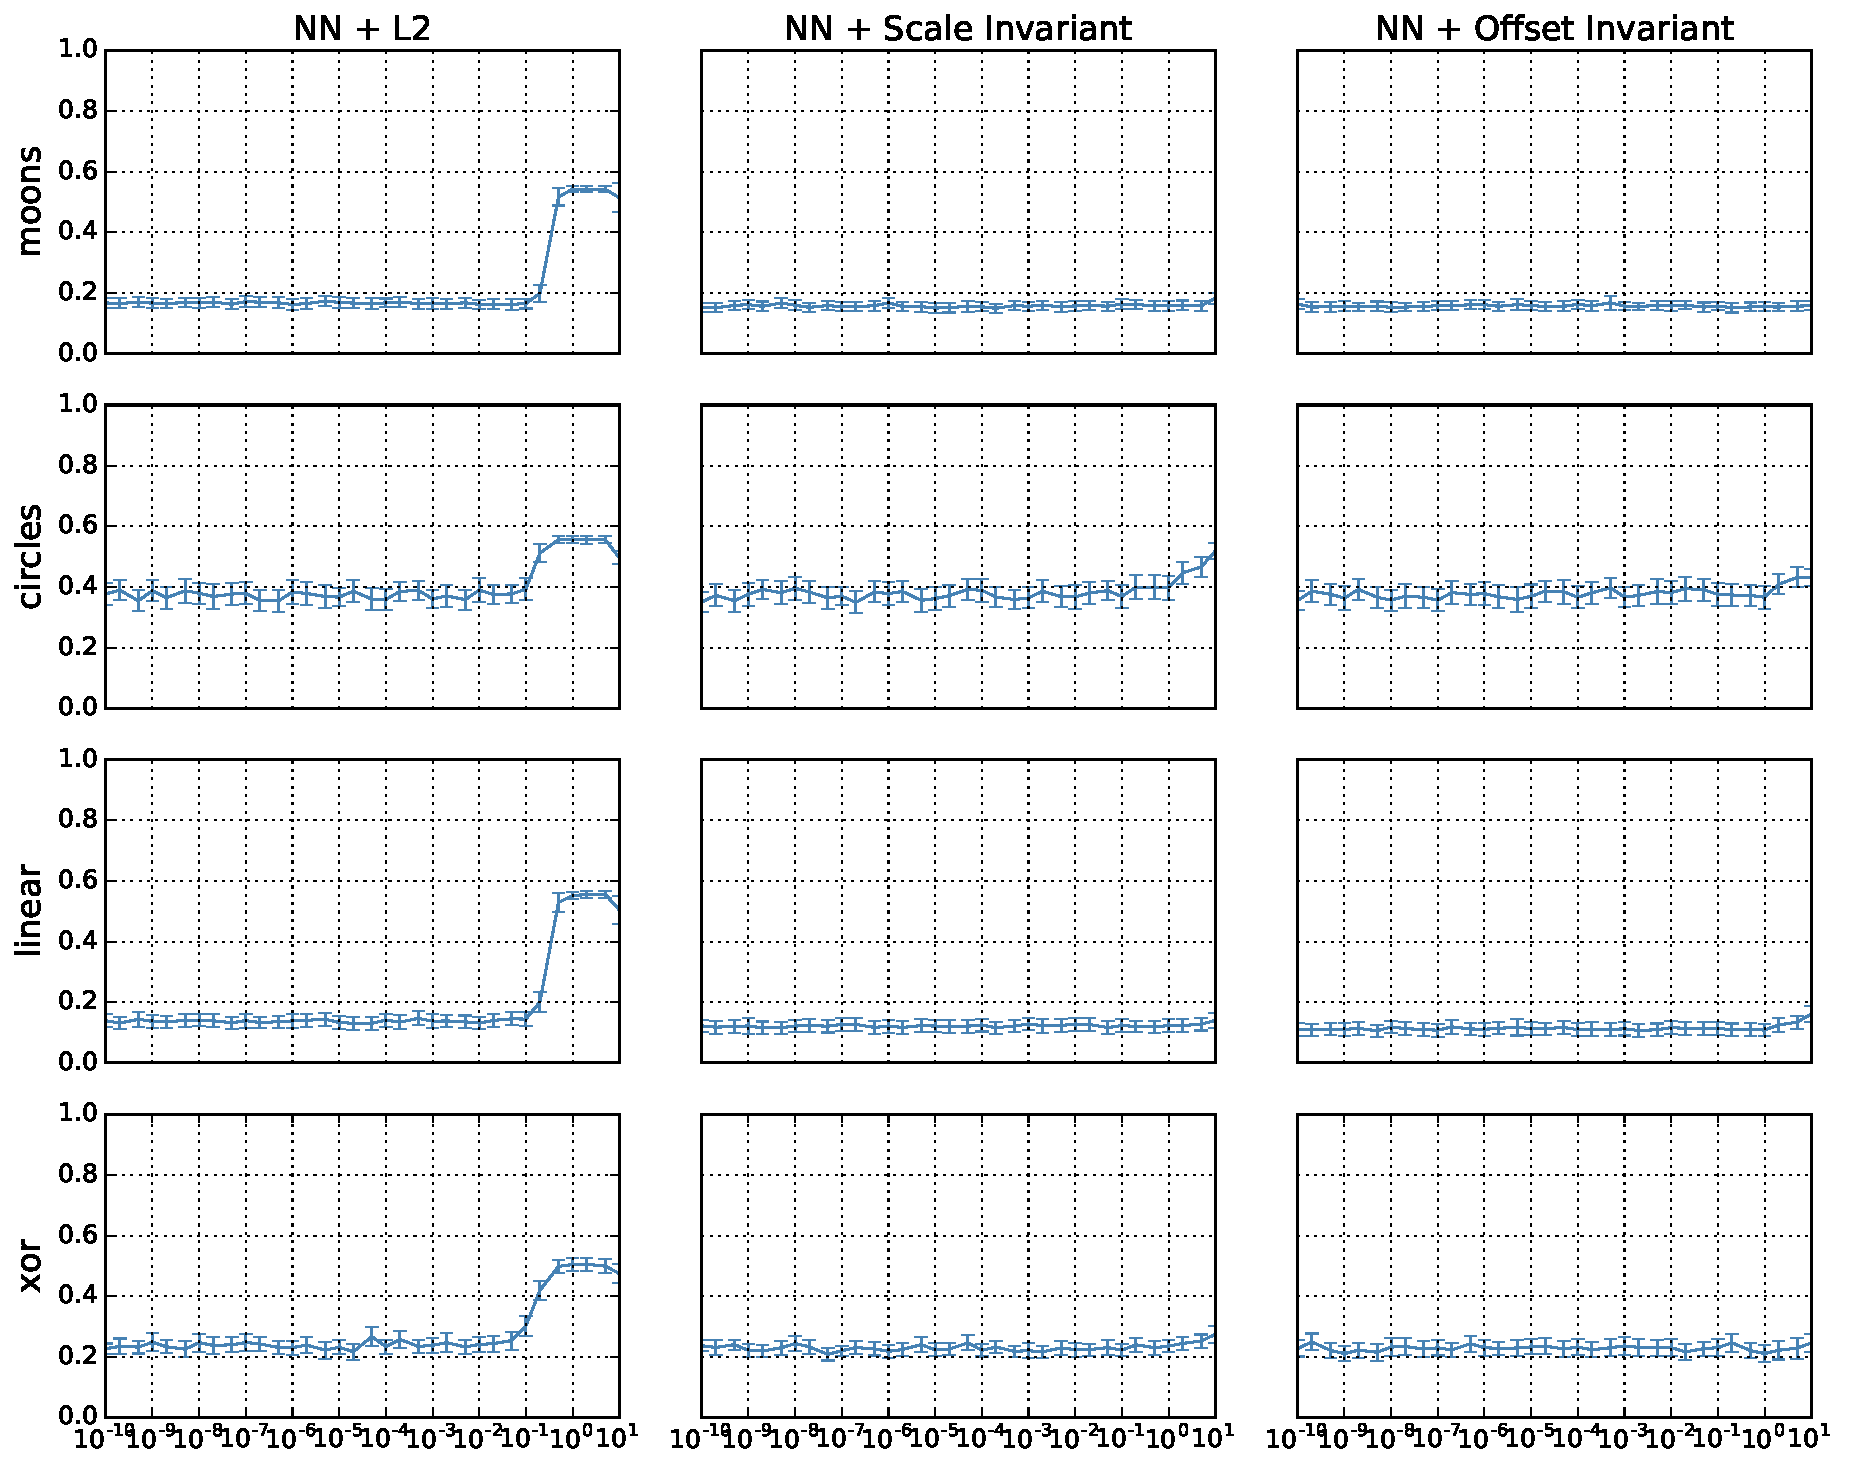
\includegraphics[width=0.7\textwidth]{plots/syntetic_reg_opt}
	\caption{Misclassification for each regularization parameter using 50 dataset for each generator and model.}
\end{figure}

\section{Contour with optimized regularization choices.}
\label{appendix:generated-contour-optimized}
\begin{figure}[H]
	\centering
	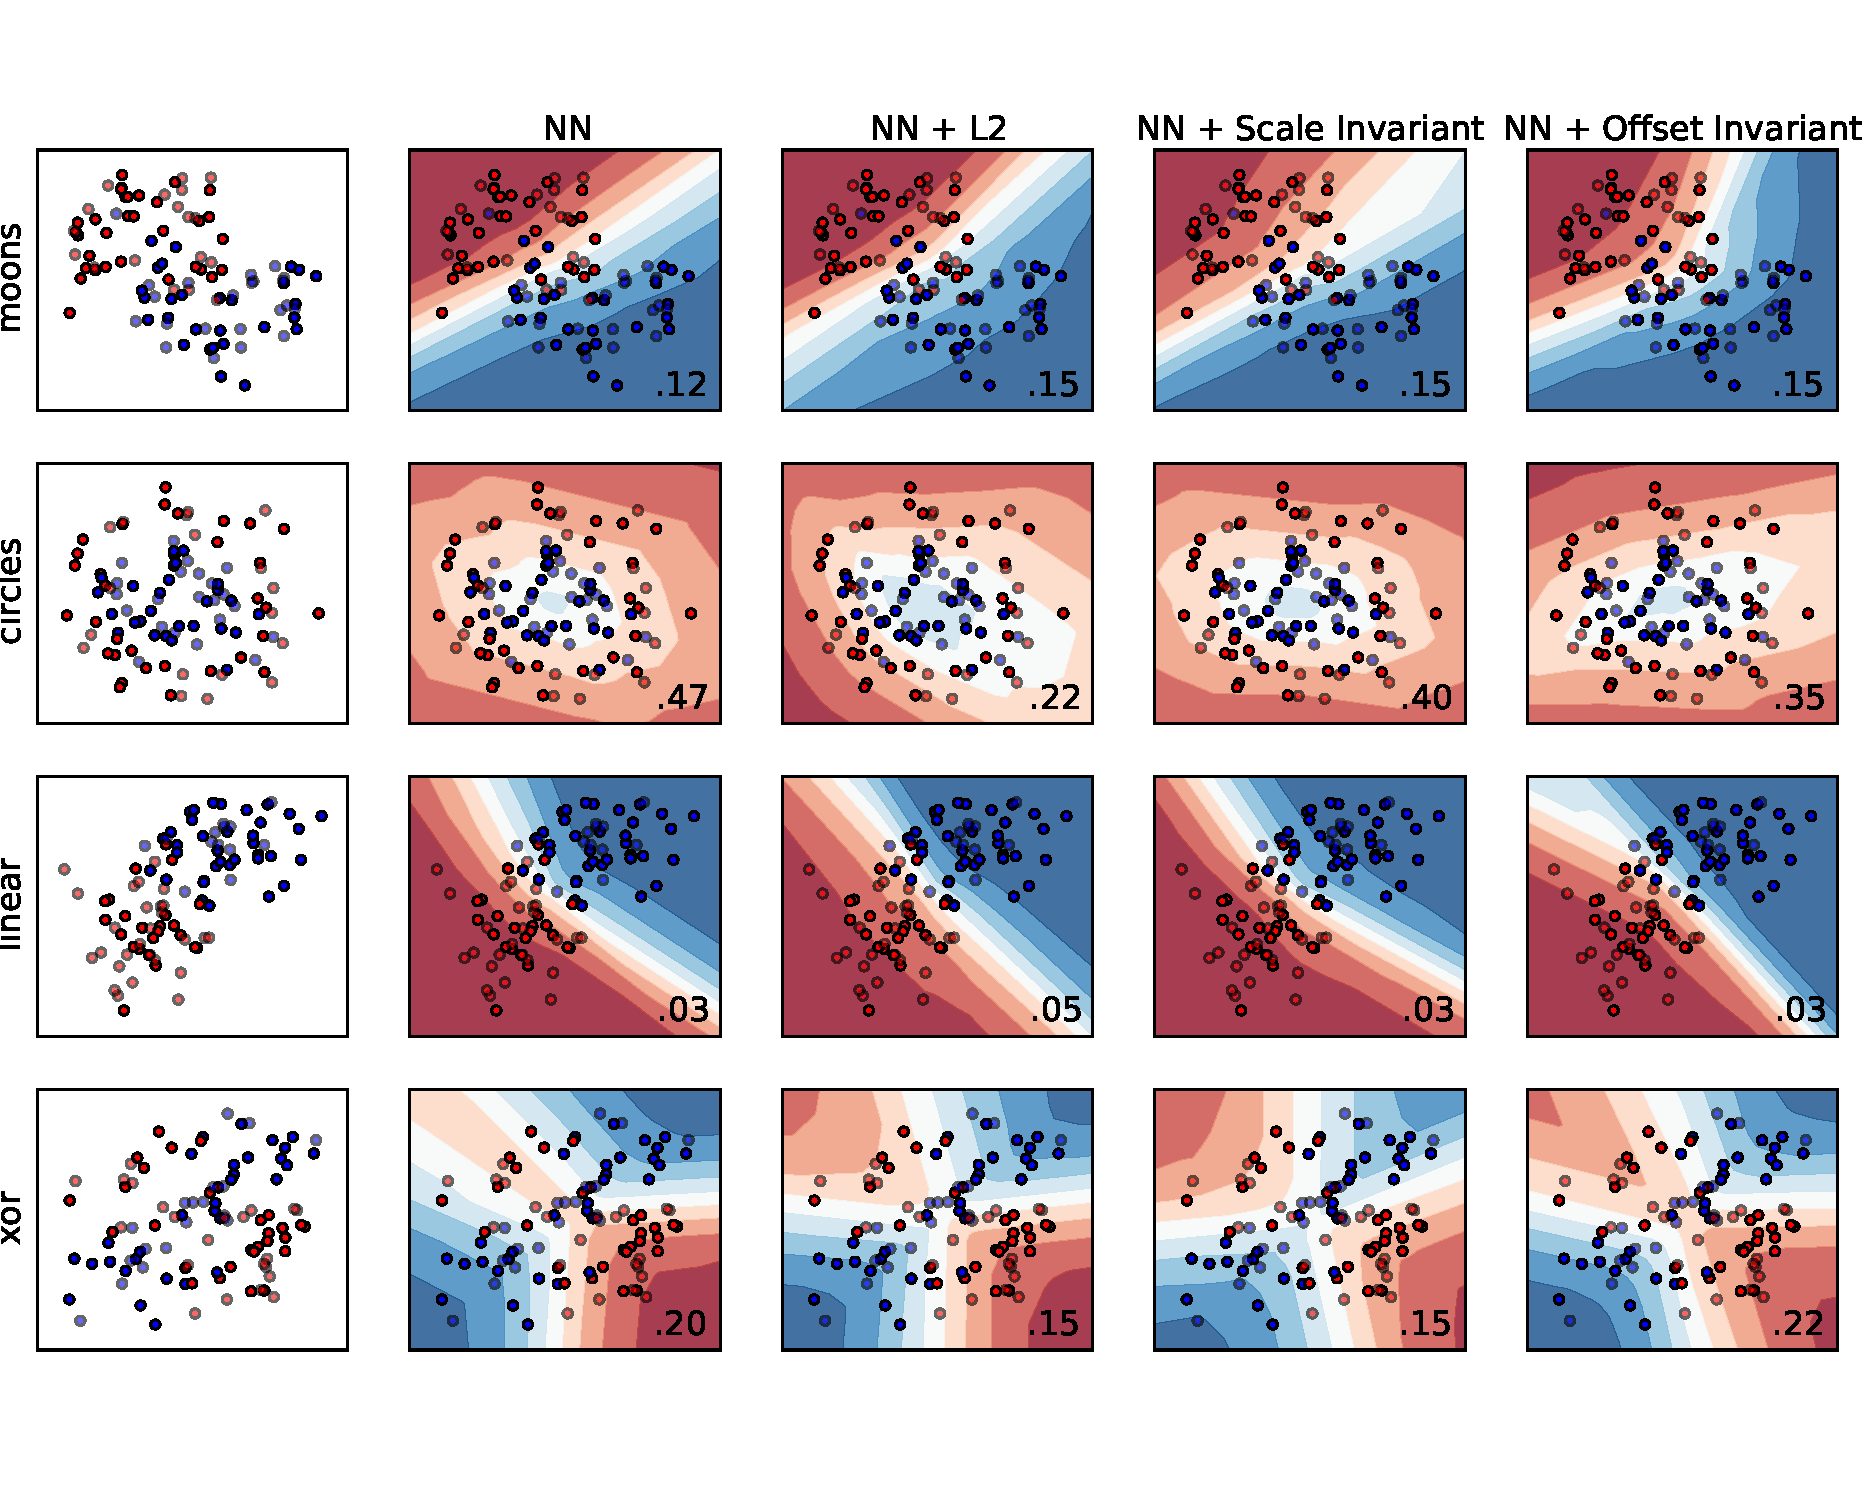
\includegraphics[width=0.7\textwidth, trim = 0 2.2cm 0 1.5cm, clip]{plots/2d_classifier-optimized}
	\caption{Contour plot of the class probability function for each classifier and dataset using optimal regularization choices.}
\end{figure}

\section{Figure}
\begin{figure}[H]
	\centering
	\includegraphics[width=1.0\textwidth]{plots/2d_alternative_example}
	\caption{Example of randomly generated observations and contour plot of the class probability function for each classifier and datagenerator}
	\label{fig:example-models}
\end{figure}

\begin{figure}[H]
	\centering
	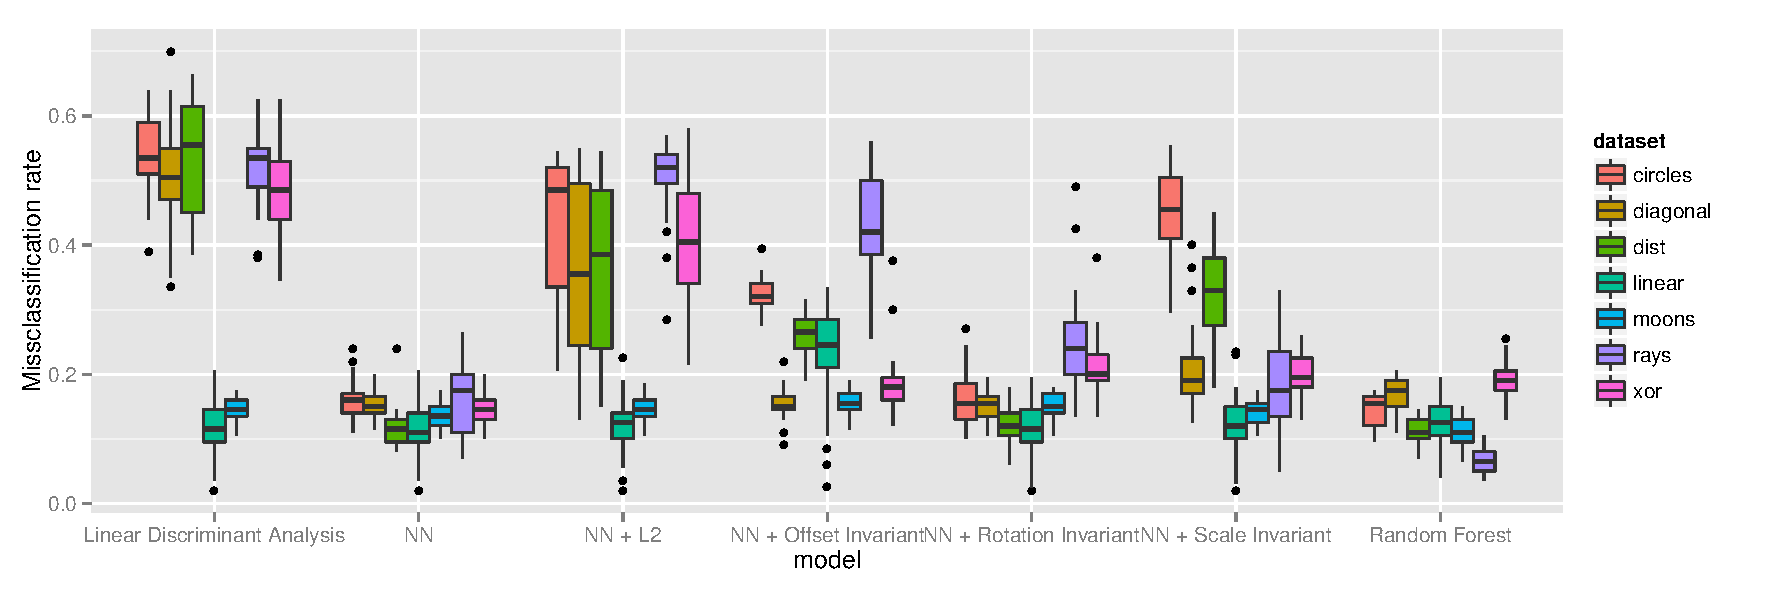
\includegraphics[width=1.0\textwidth]{plots/2d_alternative_boxplot}
	\caption{Boxplot of performance on the 25 datasets for each data generator and classification model.}
	\label{fig:boxplot}
\end{figure}

\twocolumn
\section{Weekly log}

\section{Week 4}

\subsection{Notes from meeting}

\begin{itemize}
\item What are our ambitions?
\item Neural networks are easy -> done next time
\item Neural networks are dark magic. Not very scientific approach.
\item Is it hard to predict notes from given audio data?
\end{itemize}

\subsection{For next meeting}

\textbf{Next meeting on March 1st}

\begin{itemize}
\item Read articles provided by Bjørn
\end{itemize}


\section{Week 5}

\subsection{Notes from meeting}

\begin{itemize}
\item The \textit{Sander Dieleman} article ``end-to-end learning for music
audio'' should be a good starting point.
\item Use the \texttt{timit} dataset for classification.
\item ``sensitivitet regulization'' is an interesting project direction
\item We should consider what is relevant to be invariant about. In pictures
rotational or translation invariance might make sense.
\end{itemize}

\subsection{For next meeting}

\textbf{Next meeting on March 10.}

\begin{itemize}
\item Write resume of the ``end-to-end learning for music audio'' paper.
\item Try implementing basic classification using timit data. (internal
agreement)
\end{itemize}


\subsection{Week 6}

\subsubsection{Notes from meeting}

\begin{itemize}
\item The number of bins used in our spectogram calculations are too few -> use twice the amount (approx. $100$Hz).
\item What should we do about variable input size? (length of sound files varies)
\item Too large learning rate could be a problem for converging.
\item Initialization of weights can be a major factor in convergance/performance of a network. If we want to look into steps that can be used for initializing these in a proper way, we can take a look at the 5-step process described in Jan's PhD.
\end{itemize}

\subsubsection{For next meeting}

\begin{itemize}
\item Next meeting on March 17th
\item Look into solutions to variable input size.
\item Implement CV, i.e. validate predictions
\item Normalize the input, e.g. $\log$ of spectogram (or energy/RMS-normalization)
\item Maybe add some form of regularization to the network
\end{itemize}


\section{Week 7}

\subsection{Notes from meeting}

\begin{itemize}
\item RMS-normalization of raw audio signals could be a good idea.
\item Robustness of model -> Add ``soft'' invariance regularization terms to cost function (Bjørn will be happy if we can implement this at some point).
\item A linear model using the spectrograms can be used as benchmark.
\item The book ``Digital Speech Processing'' has a section about Mel-spectrogram we can look at (not important).
\item A custom pooling layer could be a solution to varying input size.
\end{itemize}

\subsection{For next meeting}

\textbf{Next meeting on March 31th}

\begin{itemize}
\item Compare with the simple linear model.
\item Itemwise RMS normalization.
\item Think about what the model should be invariant of.
\item Look at the variance of the network output before training.
\end{itemize}


\section{Week 8}

\subsection{Notes from meeting}

\begin{itemize}
\item
\end{itemize}

\subsection{For next meeting}

\textbf{Next meeting on April 7th}

\begin{itemize}
\item
\end{itemize}


\section{Week 9}

\subsection{Notes from meeting}

\begin{itemize}
\item Sex classification is too easy a problem. Try speaker classification.
\item What tranformation function $s(x, \alpha)$ makes sense to be invariant to.
\item Transformations could be
\begin{itemize}
  \item Pitch shift
  \item Hoarse voice
  \item Noise
  \item Filter (e.g. \textit{low-pass})
\end{itemize}
\item No free lunch theorem.
\end{itemize}

\subsection{For next meeting}

\textbf{Next meeting on April 14th}

\begin{itemize}
\item Try classifying speakers instead of sex.
\item Look at audio degredation toolbox as tranformation function we want the network to be invariant to.
\item Try to implement the explicit tranformation invariance term to the loss function.
\end{itemize}


\section{Week 10}

\subsection{Notes from meeting}

\begin{itemize}
\item Create our own dataset of speakers represented $x$ number of times.
\item Make sure to cross validate the errors, when the final results are being made.
\item Could the performance of the speaker classifier be compared with human
performance?
\item The ELSDSR dataset could be used for speaker classification instead of the Timit.
\end{itemize}

\subsection{For next meeting}

\textbf{Next meeting on April 21th}

\begin{itemize}
\item Send code of invariance implementation to Bjørn. Write details of preprocessing used etc.
\item Regularize network for speaker classification. Try weight decay and dropout.
\item Test the invariance implementation on simple problem from UCI with a simple network before testing on Dieleman.
\item Reduce number of speakers used. E.g. only include speakers represented 10 times or more in the dataset.
\end{itemize}


\subsection{Week 11}

\subsubsection{Notes from meeting}

\begin{itemize}
\item $80-90 \%$ correct classification rate should be possible for speaker classifier.
\item Mean spectrogram with logitic regression.
\item Does the size on the dense layer limit our network? 300 output neurons vs 50 neurons in last dense layer??
\end{itemize}

\subsubsection{For next meeting}

\begin{itemize}
\item Next meeting on April 28th
\item Give Bjørn the data for speaker classification.
\item Give Bjørn access to github repository - maybe make it public.
\item Try mean spectogram on frequency axis using simple logistic regression.
\item Try binary classification - 1 vs many on speaker classification.
\end{itemize}


\subsection{Week 12}

\subsubsection{Notes from meeting}

\begin{itemize}
\item Bjørn will stop being our supervisor
\item We could not get any improvement over logistic regression by applying convolution. This should not be.
\item Trying another dataset showed the same behaviour.
\end{itemize}

\subsubsection{For next meeting}

\begin{itemize}
\item Next meeting on ``not agreed''
\item We should try a GMM model as a baseline
\item Bjørn will also try calculating a baseline
\item Look at Jan \& Corey paper to get baseline
\end{itemize}


\subsection{Week 13}

\subsubsection{Notes from meeting}

\begin{itemize}
\item Poster for the presentation should be made as a A0 paper.
\item The examiner will be allowed to ask into any topic mentioned in the presentation (including MFCC features).
\item We should think of an explanation for why Weight Decay isn't improving performance.
\item The structure of the representation should match the structure of the report. Explain from beginning to end in a coherent manner.
\end{itemize}

